%	This is written by Zhiyang Ong as a template for typesetting in LaTeX.

%	The MIT License (MIT)

%	Copyright (c) <2014> <Zhiyang Ong>

%	Permission is hereby granted, free of charge, to any person obtaining a copy of this software and associated documentation files (the "Software"), to deal in the Software without restriction, including without limitation the rights to use, copy, modify, merge, publish, distribute, sublicense, and/or sell copies of the Software, and to permit persons to whom the Software is furnished to do so, subject to the following conditions:

%	The above copyright notice and this permission notice shall be included in all copies or substantial portions of the Software.

%	THE SOFTWARE IS PROVIDED "AS IS", WITHOUT WARRANTY OF ANY KIND, EXPRESS OR IMPLIED, INCLUDING BUT NOT LIMITED TO THE WARRANTIES OF MERCHANTABILITY, FITNESS FOR A PARTICULAR PURPOSE AND NONINFRINGEMENT. IN NO EVENT SHALL THE AUTHORS OR COPYRIGHT HOLDERS BE LIABLE FOR ANY CLAIM, DAMAGES OR OTHER LIABILITY, WHETHER IN AN ACTION OF CONTRACT, TORT OR OTHERWISE, ARISING FROM, OUT OF OR IN CONNECTION WITH THE SOFTWARE OR THE USE OR OTHER DEALINGS IN THE SOFTWARE.

%	Email address: echo "cukj -wb- 23wU4X5M589 TROJANS cqkH wiuz2y 0f Mw Stanford" | awk '{ sub("23wU4X5M589","F.d_c_b. ") sub("Stanford","d0mA1n"); print $5, $2, $8; for (i=1; i<=1; i++) print "6\b"; print $9, $7, $6 }' | sed y/kqcbuHwM62z/gnotrzadqmC/ | tr 'q' ' ' | tr -d [:cntrl:] | tr -d 'ir' | tr y "\n"

%%%%%%%%%%%%%%%%%%%%%%%%%%%%%%%%%%%%%%%%%%%%%%



%%%%%%%%%%%%%%%%%%%%%%%%%%%%%%%%%%%%%%%%%%%
\chapter{Software Architecture of the {\sc Bib}\TeX\ Analytics Project}
\label{chp:SoftwareArchitectureOfTheBibTeXAnalyticsProject}


Figure \ref{fig:SoftwareArchitecture} shows the software architecture of the {\sc Bib}\TeX\ {\it Analytics} project. It shows the different packages of the {\sc Bib}\TeX\ {\it Analytics} project, as well as the classes in each package. \\

\begin{figure}[h]
\centering 
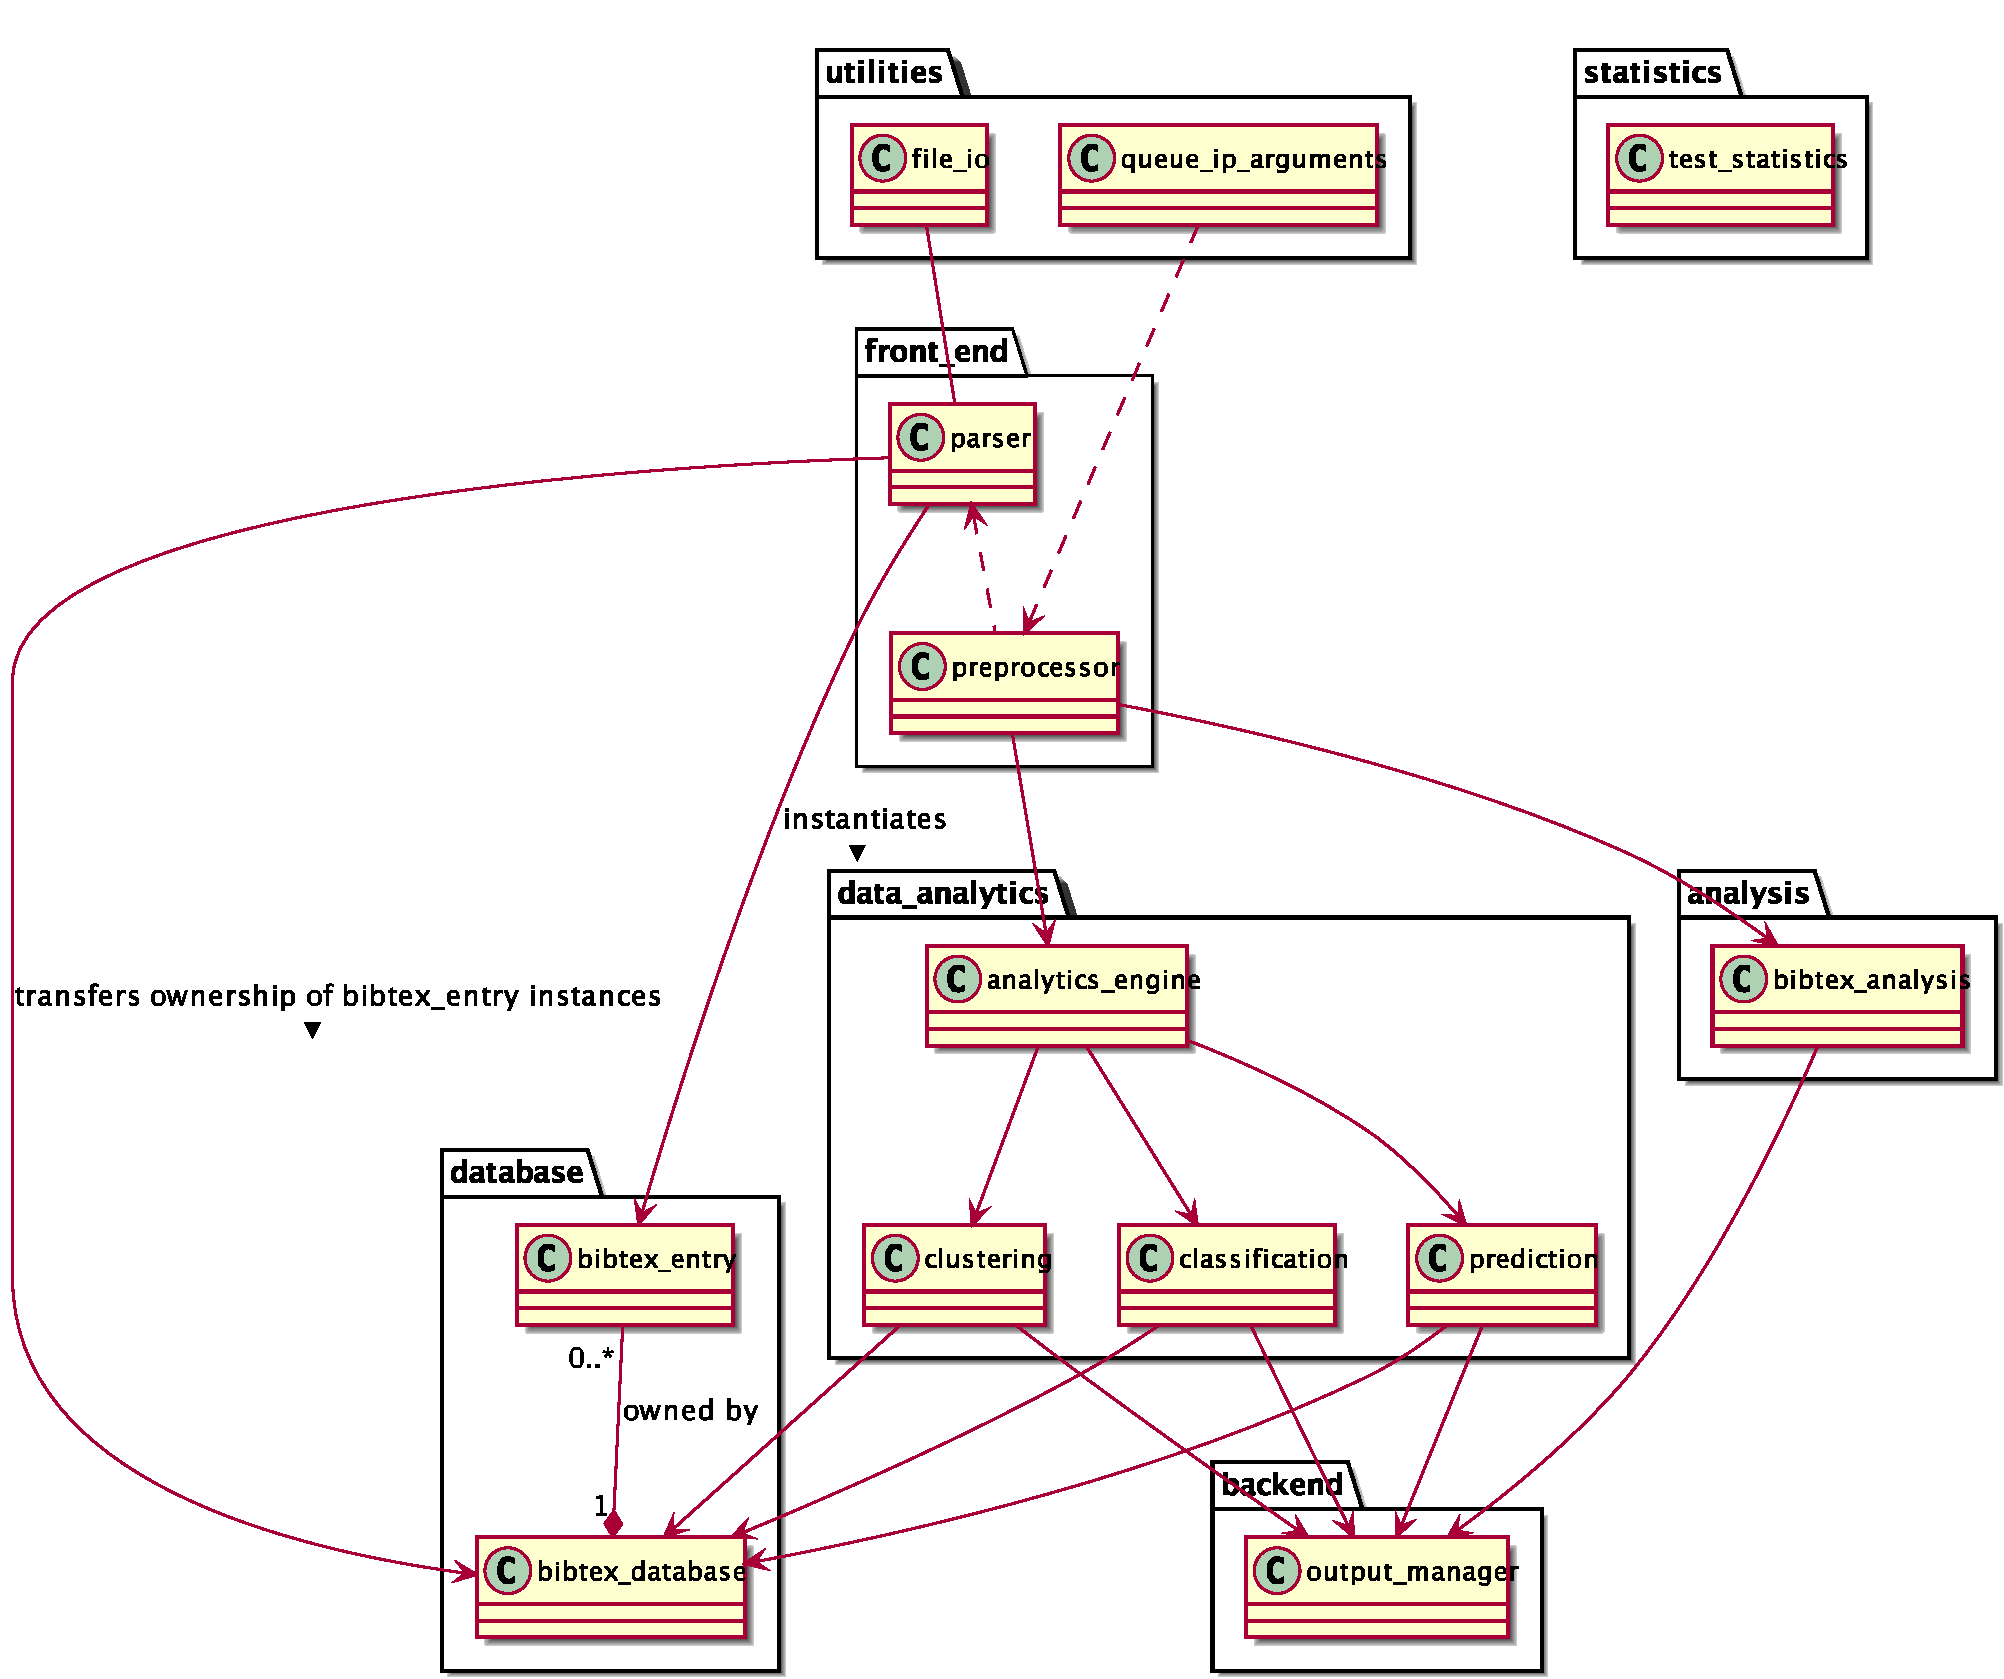
\includegraphics[height=4in]{pics/sw-arch/sw-arch}
\caption{Software architecture of the {\sc Bib}\TeX\ {\it Analytics} project.}
\label{fig:SoftwareArchitecture}
\end{figure}

The {\tt front\_end} package performs the following operations: interacts with the {\tt utilities} package to process command-line input arguments from the user and parse a {\sc Bib}\TeX\ file, instantiates a {\tt bibtex\_database} object to contain instances of {\tt bibtex\_entry} objects, instantiates a {\tt bibtex\_entry} object for each {\sc Bib}\TeX\ entry in the {\sc Bib}\TeX\ file, and passes {\tt bibtex\_entry} objects to the {\tt bibtex\_database} object for storage. Hence, this package also interacts with the {\tt database} package. Using input from the command-line input arguments, it either calls static methods of classes in the {\tt data\_analytics} package or the {\tt analysis} package. \\

When objects in the {\tt data\_analytics} package or the {\tt analysis} package performs operations specified by the command-line input arguments, it interacts with the {\tt bibtex\_database} object in the {\tt database} package to access required information to perform the aforementioned operations. When these operations are completed, objects from either of these packages, {\tt data\_analytics} or {\tt analysis}, pass the computation results to the {\tt output\_manager} in the {\tt backend} package. The {\tt output\_manager} either prints the computation results to a text file in the current working directory or to standard output for display on the {\it Terminal} application. \\

In the {\tt utilities} package, the {\tt queue\_ip\_argument} class has static methods to process command-line input arguments from the user. Likewise, the {\tt file\_io} class has static methods to process an input {\sc Bib}\TeX\ file, which is specified by the user in the command line. \\

Regarding the {\tt data\_analytics} package, the {\tt analytics\_engine} class manages the operations in data analytics, and calls the appropriate machine learning tool. The machine learning tools are: {\tt clustering}, {\tt classification}, and {\tt prediction}.

Figure \ref{fig:SoftwareArchitectureWithHigherCoupling} with highly coupled {\tt test\_statistics} class.











\begin{figure}[h]
\centering 
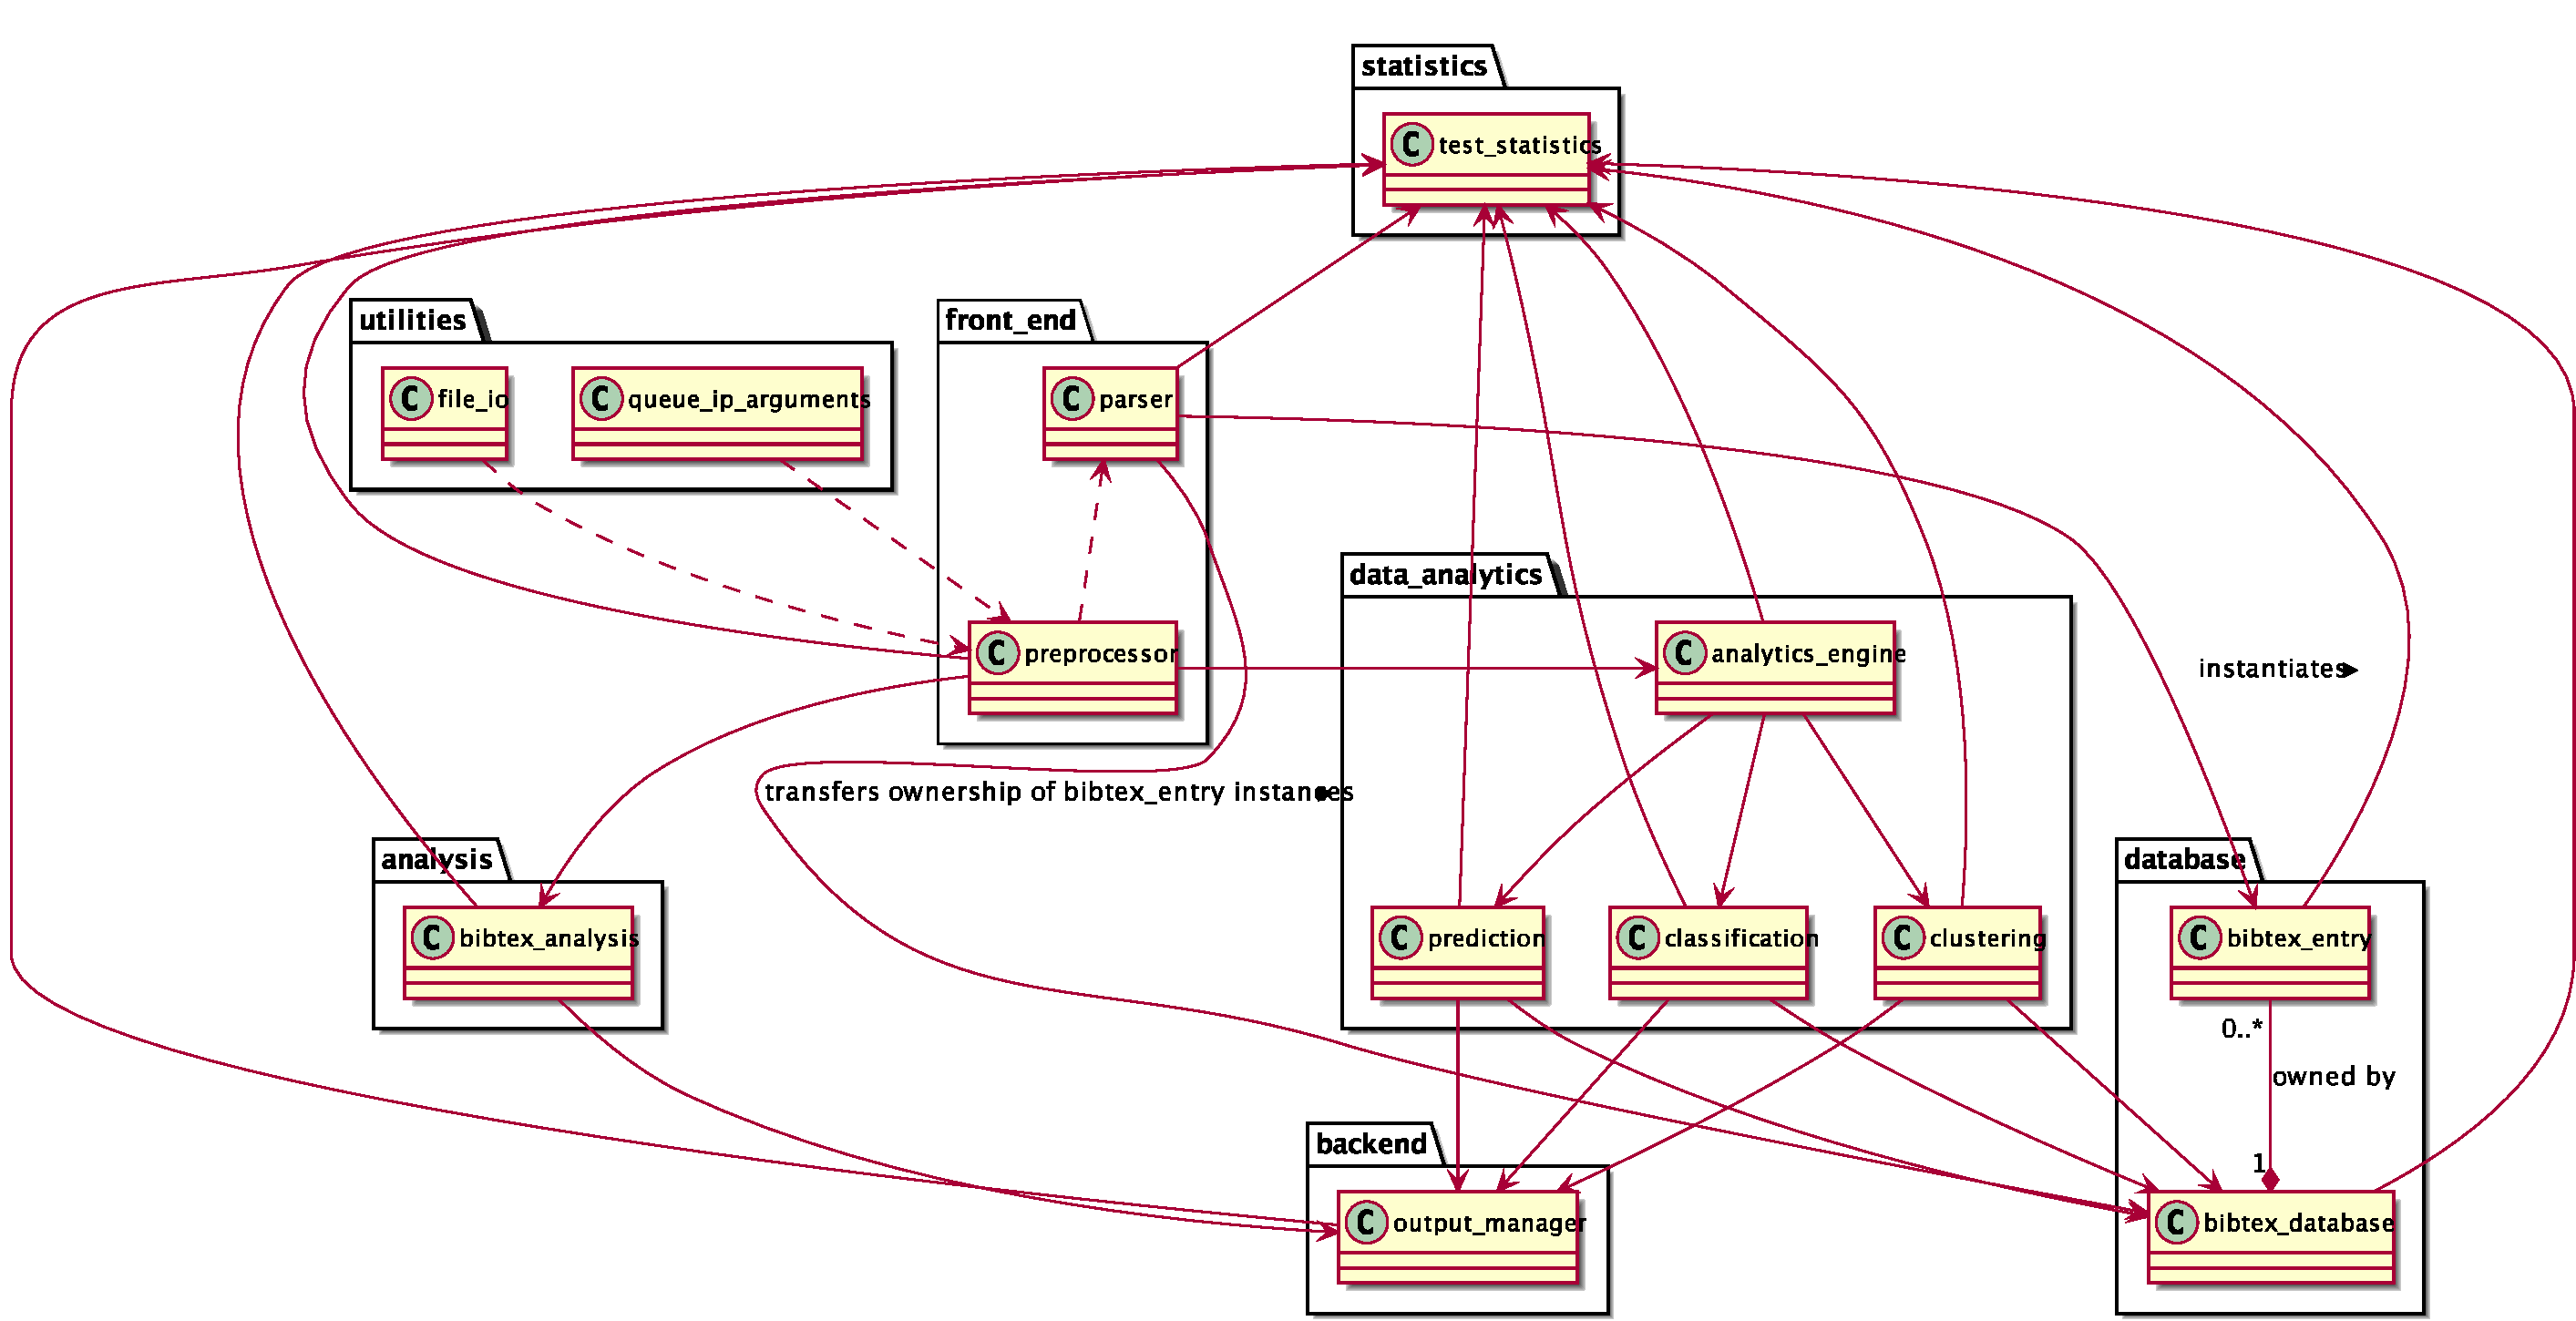
\includegraphics[height=3.5in]{pics/sw-arch-higher-coupling/sw-arch}
\caption{Software architecture of the {\sc Bib}\TeX\ {\it Analytics} project, with highly coupled {\it test\_statistics} class.}
\label{fig:SoftwareArchitectureWithHigherCoupling}
\end{figure}










































